\subsection{Registrierung und Login}
Das Klassendiagramm zeigt die drei zentralen Servlets für Registrierung und Anmeldung: \texttt{RegisterServlet}, \texttt{MitgliedLoginServlet} und \texttt{MitarbeiterLoginServlet}. Alle drei erben von \texttt{HttpServlet} und greifen über eine gemeinsame \texttt{DataSource} auf dieselbe MariaDB-Datenbank zu. Das \texttt{RegisterServlet} überschreibt \texttt{doPost()}, da die Registrierungsdaten per POST übertragen werden; die beiden Login-Servlets überschreiben stattdessen \texttt{doGet()}, um die eingegebenen Anmeldedaten zu verarbeiten.
\begin{figure}[H]
    \centering
    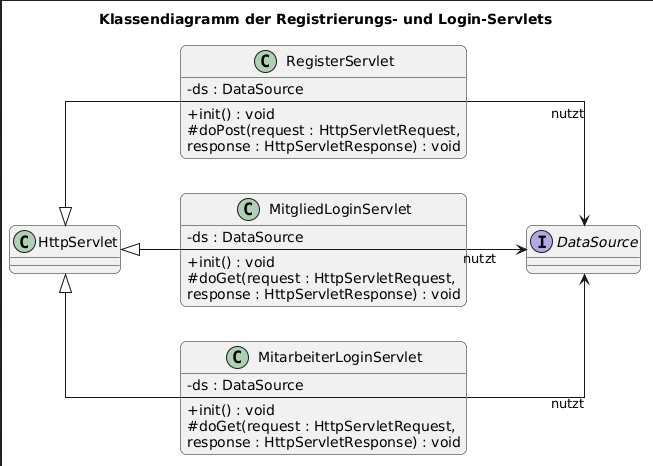
\includegraphics[width=1\linewidth]{src/abbildungen/Poster_Klassendiagramm.png}
    \caption{Klassendiagramm: RegisterServlet, MitgliedLoginServlet und MitarbeiterLoginServlet}
\end{figure}
Das \texttt{RegisterServlet} prüft zunächst, ob alle Eingaben vollständig sind und die beiden E-Mail-Felder übereinstimmen. Da zum Zeitpunkt des Einfügens die künftige Datenbank-ID noch nicht bekannt ist, wird das Mitglied zunächst mit einem Platzhalter für die Ausweisnummer angelegt und diese anschließend anhand der automatisch generierten ID nachgetragen. Die gesamte Operation läuft innerhalb einer Transaktion: Tritt ein Fehler auf, wird sie vollständig zurückgesetzt, sodass kein Mitglied mit unvollständigen Daten in der Datenbank verbleibt.
\begin{minted}{java}[h]
insertStmt.setString(5, "TEMP");
insertStmt.executeUpdate();
long generatedId;
try (ResultSet keys = insertStmt.getGeneratedKeys()) {
    keys.next();
    generatedId = keys.getLong(1);
}
String ausweisnummer = String.format("M-%06d", generatedId);
try (PreparedStatement updateStmt = connection.prepareStatement(
        "UPDATE mitglied SET ausweisnummer = ? WHERE id = ?")) {
    updateStmt.setString(1, ausweisnummer);
    updateStmt.setLong(2, generatedId);
    updateStmt.executeUpdate();
}
connection.commit();
\end{minted}
Das \texttt{MitgliedLoginServlet} vergleicht die eingegebene E-Mail-Adresse und das Passwort mit den gespeicherten Daten. Bei erfolgreicher Anmeldung wird eine Session mit Mitglieds-ID, Ausweisnummer und Rolle angelegt, bevor das Mitglied auf sein Dashboard weitergeleitet wird. Das \texttt{MitarbeiterLoginServlet} funktioniert nach demselben Prinzip, leitet nach erfolgreicher Anmeldung jedoch abhängig von der Rolle entweder auf die Administrator- oder auf die Mitarbeiterseite weiter.
